

\begin{frame}
	Frage : Gibt es $\NP$  Probleme , die nicht \NP -vollständig sind , aber auch nicht in $\P$  liegen
\end{frame}
\begin{frame}{\NP -intermediate}
	\begin{figure} 
		%\centering 
		\caption[NP-Intermediate]{$\NP$-Intermediate} 
		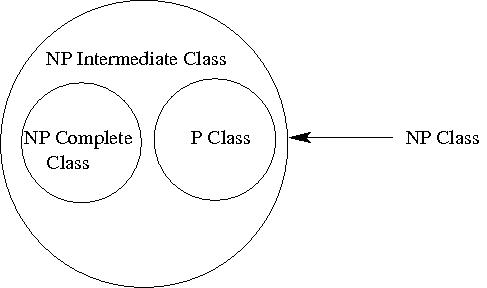
\includegraphics[scale = 0.4]{images/np-intermediate} 
		\newline 
		\label[http://functionspace.org/articles/28/Complexity-Zoo] 
	\end{figure}
\end{frame}
\begin{frame}{\NP -intermediate Probleme}
	Mögliche Kandidaten :
	\begin{itemize}
	\item Graphisomorphie (kommt in Vortrag 7)
	\item Faktorisierungsproblem
	\item Kein "natürlicher" Kandidat bekannt
	\end{itemize}
	
	aber,
\end{frame}

\begin{frame}{Satz von Ladner}
	\framesubtitle{Behauptung}
	\begin{KITinfoblock}{Existenz einer \NP -intermediate Sprache, Ladner, 75}
	Wenn $\P \neq \NP$ dann gilt : \newline
	Es existiert eine Sprache $L \in \NP \setminus \P$ die nicht \NP -vollständig ist
	\end{KITinfoblock}
\end{frame}
\begin{frame}{Beweis von Ladner}
	\framesubtitle{Beweisidee}
	Wollen eine Sprache konstruieren mit diesen Eigenschaften und zeigen, dass sie in $\NP$ - intermediate ist, falls $\P \neq \NP$  :
	
	\bigskip
	\pause
	\begin{KITinfoblock}{Die Sprache ${\SAT}_H$}
		Für eine Funktion $H$ : $\mathbb{N} \rightarrow \mathbb{N}$ definieren wir : \newline 	
		${\SAT}_H = \lbrace \psi 01^{n^{H(n)}} : \psi \in \SAT$ und $ n = |\psi| \rbrace$
	\end{KITinfoblock}
	\bigskip
	\pause	
	
	\begin{KITexampleblock}{Beispiel für ${\SAT}_H$}
	F\"ur $H(n) = n - 1$ und $\psi = a \land b$ gilt : \newline
	$(a \land b) 01^{3^2} = (a \land b) 0111111111 \in {\SAT}_H $
	\end{KITexampleblock}
	\pause
	\bigskip
	${\SAT}_H$ ist also $\SAT$ mit 1er padding
\end{frame}

\begin{frame}{Beweis von Ladner}
	\framesubtitle{Lemma}
	Wir müssen nun also $H$ geschickt wählen !
	\pause
	\begin{KITblock}{Eigenschaft, die wir von H wollen}
		${\SAT}_H \in \P \Leftrightarrow H(n) \in O(1)$ (also $H(n) \leq C$ f\"ur alle n) 				\newline
		und damit insbesondere $\lim_{n \to \infty}  H(n) = \infty$ f\"ur ${\SAT}_H
		\notin \P$
		
	\end{KITblock}	
\end{frame}
\begin{frame}{Beweis von Ladner}
	\framesubtitle{Nachweis der Eigenschaften von H}
 	\begin{KITinfoblock}{Definition von H}
		$H(n)$ ist die kleinste Gödelnummer $i < \log (\log (n))$ so dass für alle
		$ x \in \{0,1\}^*$ mit $|x| \leq \log(n) $ die Turing Maschine $M_i$ genau ${\SAT}_H(x)$
		in $i|x|^i$ Schritten berechnet. Falls dieses $i$ nicht existiert setzen wir 
		$H(n) = \log(\log(n))$ 
	\end{KITinfoblock}
	\pause
	
	\begin{overprint}
		\only<2-5> {
			\bigskip
		Zuerst zeigen wir : ${\SAT}_H \in \P \Rightarrow H(n) \in O(1)$
		\pause
		\begin{itemize}[<+->]
			\item ${\SAT}_H \in \P \Rightarrow \exists$ Turing Maschine $M$, die
			${\SAT}_H$ in höchstens $cn^c$ Schritten entscheidet.
			\item $\exists i > c$ , so dass $M_i$ = M
			\item Für n > $2^{2^i}$ gilt $H(n) \leq i$ und damit $H(n) \in O(1)$ 
		\end{itemize}
		}
		\only<6-> {
			\bigskip
			Nun : $ H(n) \in \mathcal{O}(1) \Rightarrow {\SAT}_H \in \P$
			\pause
			\begin{itemize}
				\item<7-> Da $ H(n) \in \mathcal{O}(1)$ ist Bild von $H$ endlich $ \Rightarrow \exists i$ mit $H(n) = i$ für unendlich viele $n$
				\item<8-> TM $M_i$ löst ${SAT}_H$ in $ in^i$ Schritten
				\item<9-> Denn, angenommen $\exists x$ für welches $M_i$ dies nicht in dieser Grenze schafft $\Rightarrow$ $H(n) \neq i$ für alle $ n > 2^{|x|} $
				nach Definition von $H$
				
			\end{itemize}
		
		}
	\end{overprint}
	
	
\end{frame}
\begin{frame}{Beweis von Ladner}
	\framesubtitle{${\SAT}_H$ weder in $\P$ noch  $\NP$-complete}
	\begin{KITinfoblock}{Definiton von ${SAT}_H$}
		Für eine Funktion $H$ : $\mathbb{N} \rightarrow \mathbb{N}$ definieren wir : \newline 	
		${\SAT}_H = \lbrace \psi 01^{n^{H(n)}} : \psi \in \SAT$ und $ n = |\psi| \rbrace$
	\end{KITinfoblock}
	\bigskip
	\heading{${\SAT}_H$ ist nicht in $\P$}
	\pause
	\bigskip
	\begin{itemize}[<+->]
		\item Angenommen ${\SAT}_H \in \P \Rightarrow $  $H(n) \le C$, $C$ Konstante wegen des gerade bewiesenen Lemmas
		\item ${\SAT}_H$ ist also $\SAT$  mit höchsten $n^C$  angehänten 1en
		\item $\SAT$ kann somit durch dieselbe TM gelöst werden $\Rightarrow \P = \NP$
	\end{itemize}
	
\end{frame}

\begin{frame}{Beweis von Ladner}
		\framesubtitle{${\SAT}_H$ weder in $\P$ noch $\NP$-complete}
	
		\begin{KITinfoblock}{Definiton von ${\SAT}_H$}
			Für eine Funktion $H$ : $\mathbb{N} \rightarrow \mathbb{N}$ definieren wir : \newline 	
			${\SAT}_H = \lbrace \psi 01^{n^{H(n)}} : \psi \in \SAT$ und $ n = |\psi| \rbrace$
		\end{KITinfoblock}
		
		
		\bigskip
		\only<2->{\heading{${\SAT}_H$ ist nicht $\NP$-complete}}
		
		\bigskip
		\pause
		\begin{itemize}[<+->]
		\item Angenommen ${\SAT}_H \in \NP-complete \Rightarrow $ es existiert poly. Reduktion $f$ von $\SAT$ auf ${\SAT}_H$ in $\mathcal{O}(n^i)$
		\item Da ${\SAT}_H \notin \P $ geht $H$ gegen $\infty$ 
		\item $\SAT$-Instanz $\varphi$ wird mit $f$ auf ${\SAT}_H$-Instanz der Form $\psi01^{n^{H(n)}}$ abgebildet und mit $ f \in \mathcal{O}(n^i)$ folgt \newline
		$|\psi| + {|\psi|}^{H(|\psi|)}$ und damit $|\psi| \in o(n)$
		\item Wegen $\psi| \in o(n)$ existiert dann ein Polynomialzeitalgorithmus für $\SAT$ und damit $\P = \NP$  $\Rightarrow$ Widerspruch! 
		
		\end{itemize}
\end{frame}